%!TEX encoding = UTF-8 Unicode
\documentclass[t,aspectratio=169,table]{beamer} 
% Option t              Place text of slides at the (vertical) top of the slides.
% Option handout        Ein PDF ohne Pausen und Overlayeffekte erzeugen.
% Option aspectratio=43 169 => 16:9, 1610 => 16:10, 43 => 4:3
\usepackage[utf8]{inputenc}
\usepackage[ngerman]{babel}
\usepackage{graphicx,xcolor}
\usepackage[T1]{fontenc} % 8-Bit-Zeichen; ermöglicht korrektes Kopieren von Umlauten aus dem pdf 

% SVS-Theme benutzen
\usetheme{svs2021}

\usepackage{booktabs}

\setlength{\arrayrulewidth}{0.1mm}
\setlength{\tabcolsep}{4pt}
% \renewcommand{\arraystretch}{1.5}
\renewcommand{\arraystretch}{1}

\usepackage[
    style=alphabetic,
    backend=biber,
    %backref=true
    ]{biblatex}             % Biblatex mit alphabetischem Style und biber.

\addbibresource{thesis.bib}

\DeclareFieldFormat*{title}{
    \mkbibemph{#1}}         % Make titles italics


% ===================================Dokument===================================


% \title{On using privacy preseving machine learning for\\decentralized web bot detection}
\title{On Machine Learning Based Bot Detection Using Mouse Dynamics and Request Metadata in a Practical Context}
\author{Matz-Jona Radloff}
\date{22.09.2022} % Falls ein bestimmtes Datum eingesetzt werden soll, einfach
                    %  diese Zeile aktivieren.

\begin{document}


\section{Bachelor Thesis}
\begin{frame}
\maketitle
\end{frame}

\section{Outline}
\begin{frame}
\frametitle{Outline}

\tableofcontents
\end{frame}

\section{Motivation}
\begin{frame}
\frametitle{Motivation}

\begin{itemize}
    \item (web) bot detection
    \item realistic conditions
    \item goal of being practical
\end{itemize}

\end{frame}

\section{Background}

\subsection{Bot Detection}
\begin{frame}
\frametitle{Bot Detection}

\begin{itemize}
    \item differentiate human from computer automated actors
    \item here, web bots are defined as software that automatically performs HTTP(S) request to gather information or reach a goal
    \item deny bots with malicious intentions, e.g.
    \begin{itemize}
        \item Denial of Service (DoS)
        \item Data Scrapers
        \item Content Spam
        \item Scalping
    \end{itemize}
    \item 27.7\% of all 2021 internet traffic generated by malicious bots \cite{BAD_BOT_REPORT2022}
    \item good bot traffic desired to be allowed (e.g. search engine index bots)
    \item false positive intolerant
\end{itemize}

\end{frame}

\section{Related Work}

\subsection{Previous Works}
\begin{frame}
\frametitle{Previous Works}

\begin{itemize}
    \item Iliou et al. \cite{10.1145/3339252.3339267} compare different machine learning algorithms on request metadata
    \begin{itemize}
        \item one year of request data from MK-Labs's public web server\footnote{Multimedia Knowledge and Social Media Analytics Laboratory, \url{https://mklab.iti.gr/}}
        \item derived features, e.g. percentage of image requests, number of bytes per session
        \item best machine learning methods are Random Forest and Multilayer Perceptron
        \item simple vs advanced bots, AUC of 1.00 and 0.64
    \end{itemize}
    \item Acien et al. \cite{Acien2020BeCAPTCHAMouseSM} use biometric features in a ML system for bot detection
    \begin{itemize}
        \item GAN-base mouse trajectory synthesis for training and evaluation
        \item Random Forest best ML algorithm
        \item 98.7\% accuracy
    \end{itemize}
    %\item Several works showed the potential viability of user authentication via mouse dynamics
\end{itemize}

\end{frame}

\subsection{Requirements and thesis contribution}
\begin{frame}
\frametitle{Requirements and thesis contribution}

\begin{itemize}
    \item direct comparison of ML systems using request metadata and mouse dynamics data
    \item real world conditions.
    \begin{itemize}
        \item many previous works data collection and/or evaluation in lab setting
    \end{itemize}
    \item good performance (low FPR weighed highest) and execution speed
    \item above requirements have been shown to be viable separately but not together in a practical setting
\end{itemize}

\end{frame}

\section{Method}

\subsection{Request Metadata and Mouse Dynamics for Bot Detection}
\begin{frame}
\frametitle{Request Metadata and Mouse Dynamics for Bot Detection}

\begin{columns}
\column{0.4\textwidth}
\begin{itemize}
    \item comparison of mouse and touch data to request metadata
    \item mouse data contains a lot of information and harder to fake
    \item big part of request metadata redundant, e.g. user agent
\end{itemize}

\column{0.6\textwidth}
\begin{figure}
    \includegraphics[width=\textwidth]{figures/user_mouse_heatmap.png}
    \caption{Mouse movements captured from a human user}
    %\label{fig:user_mouse_heatmap}
\end{figure}

\end{columns}

\end{frame}

\begin{frame}
\frametitle{Request Metadata and Mouse Dynamics for Bot Detection}

\begin{itemize}
    \item ML-based system is chosen because of its good performance in previous works and privacy friendliness
    \item limit scope to binary classification (only bot or human)
    \item smaller set of input features to increase execution speed and reduce complexity
    \item dataset collected and bot data generated using real websites
    \item comparison to existing dataset from Antal et. al's publication \cite{9111596}
\end{itemize}

\end{frame}

\subsection{Machine Learning Model}
\begin{frame}
\frametitle{Machine Learning Model}

\begin{itemize}
    \item previous works showed that the Random Forest algorithm performs best for both data types
    \begin{itemize}
        \item supervised ML algorithm
        \item ensemble of decision trees (reduces overfitting compared to single tree)
        \item decision tree nodes split data according to a binary decision criterion
        \item bagging of input data (per tree and node)
        \item tree's results are averaged for final prediction
        \item variable parameters (\# trees, \# features per tree, max tree depth, etc)
    \end{itemize}
\end{itemize}

\end{frame}

\subsection{Request Data Feature Selection}
\begin{frame}
\frametitle{Request Data Feature Selection}

\begin{itemize}
    \item Iliou et al. \cite{10.1145/3339252.3339267} ranked the best performing metrics
    \item the following, most applicable, subset is used
    \begin{itemize}
        \item \% of HTTP requests that returned 4xx
        \item \% of HTTP requests that returned a CSS file
        \item \% of HTTP requests that returned a JavaScript file
        \item \% of requested URLs that contain the previously requested URL as a subpart
        \item seconds between the first and the last HTTP request of the session
        \item standard deviation of requested pages' depth (i.e. number of "/" in URL path)
        \item mean and standard deviation of times between successive requests
    \end{itemize}
\end{itemize}

\end{frame}

\subsection{Mouse Data Feature Selection}
\begin{frame}
\frametitle{Mouse Data Feature Selection}

\begin{itemize}
    \item relative $x$- and $y$-coordinates, and time value
    \item grouped into paths (click at the end, max 50 datapoints or 2 seconds long)
    \item resampled such that all values or uniformly spaced in time (every 20ms)
    \item derived features are engineered similar to Gamboa et.al.\cite{GAMBOA2004} and \cite{https://doi.org/10.1049/iet-bmt.2018.5126}
    \begin{itemize}
        \item mean, SD, min, max, max-min computed for the following vectors
        \begin{itemize}
            \item path length from origin
            \item angle of path tangent with the $x$-axis
            \item horizontal, vertical, tangential and angular velocities
            \item tangential acceleration and jerk
        \end{itemize}
        \item total time, distance, straigtness, jitter \\
    \end{itemize}
    $\rightarrow$ 49 values
\end{itemize}

\end{frame}

\subsection{Websites for Data Collection}
\begin{frame}
\frametitle{Websites for Data Collection}

\begin{itemize}
    \item two blog-style websites with login and register functionality
    \item randomly generated content
    \item hybrid between classical and SPA approach
    \item both request and mouse data recorded in parallel (by JavaScript and Python backend)
    \item recorded data + UUID + human/bot label stored in database
\end{itemize}

\end{frame}

\begin{frame}
\frametitle{Websites for Data Collection}
\begin{centering}
\begin{figure}
    \includegraphics[width=0.8\textwidth]{screenshots/fmexp1_169.png}
    \caption{The user experiment's first website}
    \label{screenshot:fmexp1}
\end{figure}
\end{centering}
\end{frame}


\subsection{Bot Data Generation}
\begin{frame}
\frametitle{Bot Data Generation}

\begin{itemize}
    \item selenium-python and puppeteer (JavaScript) libraries used for automation
    \item different screen sizes, random pauses between actions, random order of actions
    \item request, mouse and advanced mouse bots implement the following actions
    \begin{itemize}
        \item Accepting the initial prompt dialog to start the experiment
        \item Visiting the top-level pages \{About, Blog, Contact/Imprint, Login, Register\}
        \item Visiting 10 randomly selected single blog pages with a parameter for how many
        \item Visiting 100 completely randomly selected pages with a parameter for how many
        \item Registering an account
    \end{itemize}
\end{itemize}

\end{frame}

\subsection{Bot Data Generation}
\begin{frame}
\frametitle{Bot Data Generation}

\begin{columns}
\column{0.4\textwidth}
\begin{itemize}
    \item mouse bots use actual mouse movements and clicks
    \item advanced mouse bot uses bezier curve interpolation of mouse trajectories
\end{itemize}

\column{0.6\textwidth}

\begin{figure}[h]
    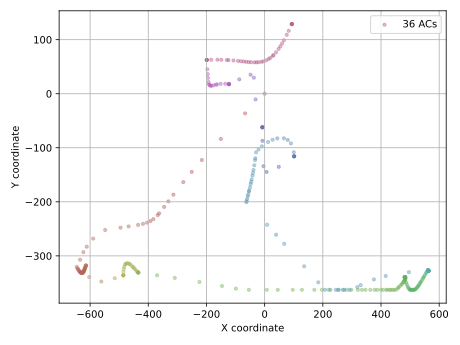
\includegraphics[width=\textwidth]{figures/bot_mouse_heatmap.png}
    \caption{Advanced Bot Mouse Movements Example}
    \label{fig:bot_mouse_heatmap}
\end{figure}
\end{columns}
\end{frame}

\section{Evaluation}

\subsection{Dataset}
\begin{frame}
\frametitle{Dataset}

\begin{itemize}
    \item 322 and 163 users participated in the experiment
    \item maximum of 10 datapoints per session as a compromise between availability and performance
\end{itemize}

\begin{figure}[h]
    \includegraphics[width=\textwidth]{figures/user_dp_hist.png}
    \caption{Distribution of users in terms of data point count}
    \label{fig:user_dp_hist}
\end{figure}

\end{frame}

\subsection{Model Hyperparameters}
\begin{frame}
\frametitle{Model Hyperparameters}

An empirical search determined the best combination of the following parameters:

\begin{itemize}
    \item Maximum number of features (None, log2, sqrt)
    \item Number of estimators (10, 50, 100, 150, 200, 1000)
    \item Maximum tree depth (None, 1, 2, 3, 4, 6, 7)
\end{itemize}
The best parameters for request data were:
\begin{table}
    \begin{center}
        \begin{tabular}{lrlrrrrr}
            Max Features & \# Trees & Max Depth & Acc. & Prec. & Recall & AUC & Tr. Time (s) \\
            \midrule
            \rowcolor{green!30}
            None & 100 & None & 0.910 & 0.887 & 0.940 & 0.973 & 0.486 \\
        \end{tabular}
    \end{center}
    \caption{Model accuracy for different parameters (request data)}
    \label{table:request_params}
\end{table}
The best parameters for mouse data were:
\begin{table}
    \begin{center}
        \begin{tabular}{lrlrrrrr}
            Max Features & \# Trees & Max Depth & Acc. & Prec. & Recall & AUC & Tr. Time (s) \\
            \midrule
            \rowcolor{green!30}
            sqrt & 200 & None & 0.966 & 0.962 & 0.970 & 0.994 & 5.899 \\
        \end{tabular}
    \end{center}
    \caption{Model accuracy for different parameters (mouse data)}
    \label{table:mouse_params}
\end{table}


\end{frame}

\section{Bibliography}
\begin{frame}
\frametitle{Bibliography}

\begin{raggedright}
  \printbibliography
\end{raggedright}

\end{frame}

\end{document}
